\chapter{Object Detection with Intel RealSense D455 Using ArUco Markers}

This chapter presents a method for object detection and pose estimation using the Intel RealSense D455 depth camera and ArUco markers. 
The approach relies on placing fiducial markers on the object of interest to facilitate accurate and robust pose estimation. 
The methodology can be divided into three main stages: creation of ArUco markers, camera calibration, and marker detection with pose estimation.

As part of this project, the implementation is available on GitHub, in the object\_det directory at the following link: 
\href{https://github.com/francy2001/relative_navigation.git}{GitHub Repository}.

\section{Intel RealSense Depth Camera D455}

The Intel\textsuperscript{\textregistered} RealSense\texttrademark\ Depth Camera D455 is a high-performance stereo depth camera that combines precision depth sensing with RGB imaging in a compact form factor. 
Its design allows for rapid integration into robotic platforms, machine vision systems, and industrial applications, making it a versatile tool for both research and development.
\\
The D455 relies on dual global shutter sensors to capture depth information using stereo vision. 
This approach enables accurate distance measurements across a range of 0.4 meters up to approximately 6 meters, depending on ambient lighting conditions. 
The depth sensor provides a resolution of up to $1280 \times 720$ pixels at 90 frames per second, while the integrated RGB sensor can capture images up to $1280 \times 800$ pixels at the same frame rate. 
This combination ensures that both geometric and visual information are available for object detection, mapping, and navigation tasks.
\\
A key feature of the D455 is its wide field of view, which exceeds 90° diagonally, allowing the camera to perceive larger portions of the environment in a single frame. 
Additionally, the camera integrates a 6 Degrees of Freedom (6DoF) Inertial Measurement Unit (IMU), providing complementary motion information that can improve stabilization, tracking, and sensor fusion algorithms.
\\
The camera is powered via a USB 3.1 Gen 1 connection, which simplifies hardware integration by providing both data transfer and power through a single cable. 
Its compact dimensions and lightweight design make it particularly suitable for mobile robots, drones, and embedded vision systems where space and weight constraints are critical.
\\
The D455 is supported by the Intel\textsuperscript{\textregistered} RealSense SDK 2.0, which is compatible with Windows, Linux, and macOS. 
The SDK offers APIs in C++, Python, and other languages, and includes tools for calibration, visualization, and integration with popular frameworks such as ROS, OpenCV, and Unity. 


\section{Object Detection}

\subsection{Creation of ArUco Markers}

To enhance the robustness of pose estimation, multiple ArUco markers are generated and attached to the object. 
The markers are created programmatically and randomly positioned on a virtual board to avoid overlapping positions. 
A sample code snippet for marker generation is shown below:

\begin{lstlisting}[basicstyle=\ttfamily\scriptsize, language=Python]
for i in range(num_markers):
    marker_id = random.randint(0, dictionary.bytesList.shape[0] - 1)
    marker_img = cv2.aruco.generateImageMarker(dictionary, marker_id, marker_size)
    # Random placement logic to avoid overlap
    # Place marker on virtual board
\end{lstlisting}

\noindent After printing, the markers are physically attached to the object to provide detectable reference points for pose estimation.

\subsection{Camera Calibration}

Accurate pose estimation requires precise knowledge of the camera intrinsic parameters. 
Calibration is performed using a standard chessboard pattern, captured in multiple poses. The corners of the chessboard are detected and refined using sub-pixel accuracy:

\begin{lstlisting}[basicstyle=\ttfamily\scriptsize, language=Python]
ret, corners = cv2.findChessboardCorners(gray, chessboard_size, None)
if ret:
    corners = cv2.cornerSubPix(gray, corners, (11, 11), (-1, -1), criteria)
    objpoints.append(objp)
    imgpoints.append(corners)
ret, mtx, dist, rvecs, tvecs = cv2.calibrateCamera(objpoints, imgpoints, gray.shape[::-1], None, None)
\end{lstlisting}

\noindent The resulting intrinsic matrix \texttt{camera\_matrix} and distortion coefficients \texttt{dist\_coeffs} are then used for marker detection and pose estimation.

\subsection{ArUco Marker Detection and Pose Estimation}

With the camera calibrated, ArUco markers are detected in the RGB images captured by the RealSense camera. 
The detection process uses a predefined ArUco dictionary and detector parameters. 
If markers are detected, their individual poses are estimated, and the axes are drawn on the image for visualization:

\begin{lstlisting}[basicstyle=\ttfamily\scriptsize, language=Python]
aruco_dict = aruco.getPredefinedDictionary(aruco_type)
parameters = aruco.DetectorParameters()
detector = aruco.ArucoDetector(aruco_dict, parameters)
corners, ids, rejected = detector.detectMarkers(gray)

if ids is not None:
    rvecs, tvecs, _ = aruco.estimatePoseSingleMarkers(corners, marker_size, mtx, dist)
\end{lstlisting}

\noindent Finally, the overall pose of the object is estimated by fusing the positions and orientations of all detected markers. 
The translation vectors are averaged, and the rotations are converted to quaternions, averaged, normalized, and converted back to rotation vectors:

\begin{lstlisting}[basicstyle=\ttfamily\scriptsize, language=Python]
if len(tvecs) > 0:
    t_fused = np.mean(np.array(tvecs), axis=0)
    quaternions = [R.from_rotvec(r).as_quat() for r in rvecs]
    quat_mean = np.mean(quaternions, axis=0)
    quat_mean /= np.linalg.norm(quat_mean)
    r_fused = R.from_quat(quat_mean).as_rotvec()
\end{lstlisting}

\noindent This fused pose provides a reliable estimate of the object's position and orientation, enabling downstream applications such as robotic manipulation or navigation in structured environments.

\begin{figure}[H]
    \centering
    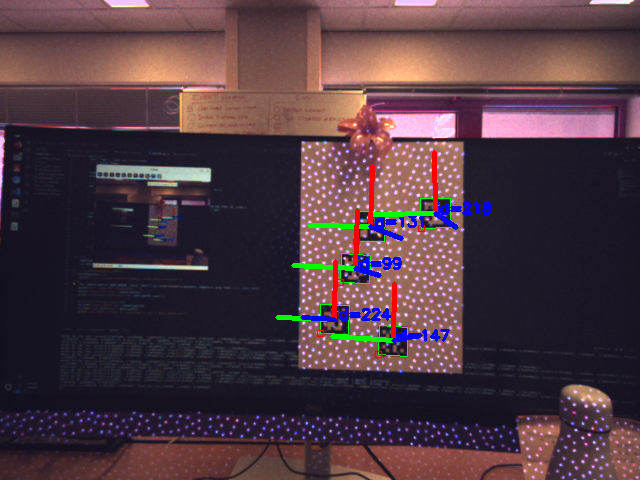
\includegraphics[width=0.6\textwidth]{figs/aruco_det.png}
    \caption{ArUco marker detection and pose estimation visualization.}
    \label{fig:aruco_detection}
\end{figure}